% \iffalse meta-comment
%<*internal>
\iffalse
%</internal>
%<*readme>
denisbdoc - A personal package for documenting classes and packages, v. 0.7
===========================================================================

**The (quick 'n dirty) `denisbdoc` package is just for documenting the classes
I've written.**

The class is supplied in `.dtx` format. If you want to unpack the `.dtx`
yourself, running:

     tex denisbdoc.dtx

will extract the package.

This package is currently not documented.
%</readme>
%<*internal>
\fi
\def\nameofplainTeX{plain}
\ifx\fmtname\nameofplainTeX\else
  \expandafter\begingroup
\fi
%</internal>
%<*install>
\input l3docstrip.tex
\askforoverwritefalse
\preamble
-----------------------------------------------------------------------------
denisbdoc --- A personal dirty package for documenting packages, version 0.7

Maintained by Denis Bitouz'e
E-mail: denis.bitouze@lmpa.univ-littoral.fr
Released under the LaTeX Project Public License v1.3c or later
See http://www.latex-project.org/lppl.txt
-----------------------------------------------------------------------------

\endpreamble
\postamble
Copyright (C) 2015, 2016, 2017 by
  Denis Bitouz'e <denis.bitouze@lmpa.univ-littoral.fr>

It may be distributed and/or modified under the conditions of
the LaTeX Project Public License (LPPL), either version 1.3c of
this license or (at your option) any later version.  The latest
version of this license is in the file:
   http://www.latex-project.org/lppl.txt

This work is "maintained" (as per LPPL maintenance status) by
  Denis Bitouz'e.

This work consists of the file  denisbdoc.dtx
                                denisbdoc.sty and
                                denisbdoc.ins.
\endpostamble
\usedir{tex/latex/denisbdoc}
\generate{
  \file{\jobname.sty}{\from{\jobname.dtx}{package}}
}
\nopreamble\nopostamble
\generate{
  \file{\jobname.xdy}{\from{\jobname.dtx}{xindy-style}}
  \file{\jobname-chng.xdy}{\from{\jobname.dtx}{xindy-style-chng}}
}
%</install>
%<install>\endbatchfile
%<*internal>
\usedir{source/latex/denisbdoc}
\generate{
  \file{\jobname.ins}{\from{\jobname.dtx}{install}}
}
\nopreamble\nopostamble
\usedir{/}
\generate{
  \file{README.md}{\from{\jobname.dtx}{readme}}
}%
\ifx\fmtname\nameofplainTeX
  \expandafter\endbatchfile
\else
  \expandafter\endgroup
\fi
%</internal>
%<*driver|package>
\RequirePackage{expl3,l3keys2e,xparse}
%</driver|package>
%<*driver>
% \documentclass[english,french]{ltxdoc}
% \usepackage{denisbdoc}
% % Silence annoying fp package messages
% %\DisableImplementation
% \begin{document}
%   \DocInput{\jobname.dtx}
% \end{document}
%</driver>
% \fi
%
% \GetFileInfo{\jobname.sty}
%
%\title{^^A
%  \textsf{denisbdoc} --- A personal package for documenting packages\thanks{^^A
%    This file describes \fileversion, last revised \filedate.^^A
%  }^^A
%}
%\author{^^A
%  Denis Bitouz'e\thanks
%    {^^A
%      E-mail: \href{mailto:denis.bitouze@lmpa.univ-littoral.fr}
%      {\texttt{denis.bitouze@lmpa.univ-littoral.fr}}^^A
%    }^^A
%}
%\date{Released \filedate}
%
%\maketitle
%
%\changes{v0.1}{2015/03/15}{First CTAN version}
%\changes{v0.2}{2016/04/04}{Second CTAN version}
%\changes{v0.3}{2016/06/10}{Third CTAN version}
%\changes{v0.4}{2016/10/24}{Fourth CTAN version}
%\changes{v0.5}{2016/10/30}{Fifth CTAN version}
%\changes{v0.6}{2016/12/08}{Sixth CTAN version}
%\changes{v0.7}{2017/01/01}{Seventh CTAN version}
%
%\begin{abstract}
% ...
%\end{abstract}
%
%\tableofcontents
%
%\begin{documentation}
%
%\section{Introduction}
%
% ...
%
%\section{Installation}
%
% The package is supplied in \file{dtx} format and as a pre-extracted
% zip file, \file{\jobname.tds.zip}. The later is most convenient for
% most users: simply unzip this in your local texmf directory and
% run \texttt{texhash} to update the database of file locations. If
% you want to unpack the \file{dtx} yourself, running
% \texttt{tex \jobname.dtx} will extract the package whereas
% \texttt{latex \jobname.dtx} will extract it and also typeset the
% documentation.
%
% The package requires \LaTeX3 support as provided in the
% \pkg{l3kernel} and \pkg{l3packages} bundles. Both of these are available
% on \href{http://www.ctan.org}{\textsc{ctan}} as ready-to-install
% zip files. Suitable versions are available in MiK\TeX{}~2.9 and
% \TeX{}~Live 2014 (updating the relevant packages online may be
% necessary). \LaTeX3, and so \pkg{denisbdoc}, requires the \eTeX{}
% extensions: these are available on all modern \TeX{} systems.
%
% Typesetting the documentation requires a number of packages in
% addition to those needed to use the package. This is mainly
% because of the number of demonstration items included in the text. To
% compile the documentation without error, you will need the packages:
%\begin{itemize}
% \item \pkg{amsmath}
% \item \pkg{booktabs}
% \item \pkg{cancel}
% \item \pkg{caption}
% \item \pkg{cleveref}
% \item \pkg{colortbl}
% \item \pkg{csquotes}
% \item \pkg{helvet}
% \item \pkg{mathpazo}
% \item \pkg{multirow}
% \item \pkg{listings}
% \item \pkg{pgfplots}
% \item \pkg{xcolor}
%\end{itemize}
%
%\end{documentation}
%
%\begin{implementation}
%
%  \chapter{Implementation}
%
%    \begin{macrocode}
%<*package>
%    \end{macrocode}
%
%    \begin{macrocode}
%<@@=denisbdoc>
%    \end{macrocode}
%
% \section{Preliminaries}
%
% The usual preliminaries.
%    \begin{macrocode}
\ProvidesExplPackage {denisbdoc} {2017/01/01} {0.7}
  {A personal package for documenting packages}
%    \end{macrocode}
%
% Make sure that the version of \pkg{l3kernel} in use is sufficiently new.
% This will also trap any problems with \pkg{l3packages} (as the two are now
% tied together, version-wise).
%    \begin{macrocode}
\@ifpackagelater { expl3 } { 2012/11/21 }
  { }
  {
    \PackageError { denisbdoc } { Support~package~expl3~too~old }
      {
        You~need~to~update~your~installation~of~the~bundles~'l3kernel'~and~
        'l3packages'.\MessageBreak
        Loading~denisbdoc~will~abort!
      }
    \tex_endinput:D
  }
%    \end{macrocode}
%
% \section{Options}
%
%    \begin{macrocode}
\keys_define:nn { denisbdoc }
{
  yad .bool_gset:N = \g_@@_yad_bool,
  gzt .bool_gset:N = \g_@@_gzt_bool,
  nwejm .bool_gset:N = \g_@@_nwejm_bool,
}
%    \end{macrocode}
%
%    \begin{macrocode}
\ProcessKeysOptions { denisbdoc }
%    \end{macrocode}
%
% \section{Packages}
%
%    \begin{macrocode}
\PassOptionsToPackage{obeyspaces}{url}
%    \end{macrocode}
%
%    \begin{macrocode}
\sys_if_engine_pdftex:TF
  {
    \RequirePackage[T1]{fontenc}
    \RequirePackage[utf8]{inputenc}
  }{
    \RequirePackage{fontspec}
  }
\RequirePackage{xpatch}%
\AtEndPreamble{%
  \RequirePackage{mweights}%
}%
%
% \let\denisbdoc@ORI@task\task
% \let\task\relax
% \RequirePackage{exsheets}
% \let\task\denisbdoc@ORI@task
\RequirePackage{parskip}%
% \RequirePackage{amsthm}%
% \RequirePackage{thmtools}%
\RequirePackage{fixfoot}%
\RequirePackage{marginnote}
\RequirePackage[inline]{enumitem}%
\RequirePackage{afterpage}%
\RequirePackage{calc}%
% \RequirePackage[lining]{libertine}%
\RequirePackage{siunitx}%
% \RequirePackage[a4paper]{geometry}%
\RequirePackage{booktabs}%
\RequirePackage{multirow}%
\RequirePackage[xr]{zref}%
\RequirePackage[multiple]{footmisc}%
% \RequirePackage[multiple,bottom]{footmisc}%
\RequirePackage{rotating}%
\RequirePackage{pdflscape}%
\RequirePackage{xspace}%
\RequirePackage{accsupp}
\RequirePackage{hologo}%
\RequirePackage{xifthen}%
\RequirePackage{refcount}%
\RequirePackage{iflang}%
\RequirePackage{ifpdf}%
\RequirePackage{amssymb}%
\RequirePackage{tocvsec2}%
\RequirePackage{ltxcmds}%
\RequirePackage{csquotes}%
\RequirePackage{tikz}%
\RequirePackage{translator}%
% \RequirePackage{scrlfile}
%
\let\EUR\relax
\RequirePackage{comment}%
\RequirePackage{path}%
\RequirePackage{textcase}%
\RequirePackage{fontawesome}%
\@ifpackageloaded{biblatex}{%
%    \end{macrocode}
%
% Réglage nécessaire sans quoi le titre courant \textquote{BIBLIOGRAPHIE}
% apparaît en trop en entête et en pied de page
%    \begin{macrocode}
\AtEndPreamble{%
  \bool_if:nT {\g_@@_yad_bool} {%
    % \defbibheading{bibintoc}[\bibname]{\chapter*{#1}}%
    % % \defbibheading{subbibintoc}[\bibname]{\section*{#1}}%
    % \defbibheading{YAD@localbibs@heading}[\translate{lbl-localbibname}]{%
    %   % \YAD@setsecnumdepth{none}%
    %   \section*{#1}%
    %   % \YAD@setsecnumdepth{\YAD@secnumdepth}%
    % }%
%    \end{macrocode}
%
% Redéfinition de la commande d'insertion de la bibliographie et ce,
% seulement si le \Package{biblatex} est chargé
% \begin{macro}{\printbibliography}
%    \begin{macrocode}
    \let\_@@_printbibliography_ORI\printbibliography%
    \renewcommand{\printbibliography}[1][]{%
      \pagestyle{biblio}%
      \_@@_printbibliography_ORI[heading=bibintoc,#1]%
      \pagestyle{ordinary}%
    }%
  }{%
  }%
}%
}{%
  \RequirePackage[backend=biber,style=authortitle,autopunct=false,useprefix=true,backref,dashed=false]{biblatex}%
}%
%    \end{macrocode}
%
% In order to as many write \enquote{streams} in auxiliary files as needed. It
% has to be loaded not too late (otherwise it cannot fix troubles it is used
% for), but not too early (otherwise the compilation stops a long time at the
% line:
% ×/usr/local/texlive/.../texmf-dist/tex/latex/latexconfig/epstopdf-sys.cfg×,
% trouble reported to the author).
%    \begin{macrocode}
\RequirePackage{morewrites}%
\RequirePackage{babel}%
% \RequirePackage[useregional]{datetime2}%
\RequirePackage[nodayofweek]{datetime}%
% \RequirePackage{floatrow}%
\RequirePackage{subcaption}%
%
% \Pkg{tocbibind} should be loaded before \pkg{imakeidx}, otherwise it would
% destroy the |\indexprologue| feature of the latter.
\RequirePackage{tocbibind}%
\RequirePackage[xindy]{imakeidx}
%
% \@ifpackageloaded{hypdoc}{%
% }{%
%   \let\oldmaketitle\maketitle
%   \RequirePackage{hypdoc}%
%   \let\maketitle\oldmaketitle
% }%
\RequirePackage{varioref}%
\@ifpackageloaded{tcolorbox}{%
}{%
  \RequirePackage{tcolorbox}%
}%
\@ifpackageloaded{hyperref}{%
}{%
  \RequirePackage[hyperfootnotes=false,hyperindex=false]{hyperref}%
}%
\RequirePackage{attachfile2} \@ifpackageloaded{nameref}{%
}{%
  \RequirePackage{nameref}%
}%
\@ifpackageloaded{hypcap}{%
}{%
  \RequirePackage[all]{hypcap}%
}%
\@ifpackageloaded{bookmark}{%
}{%
  \RequirePackage[numbered]{bookmark}%
}%
\@ifpackageloaded{glossaries}{%
}{%
  % \RequirePackage{glossaries}%
  \RequirePackage[xindy,hyperfirst=false,toc=false]{glossaries-extra}%
  \makeglossaries%
  \setglossarystyle{indexhypergroup}%
  \setabbreviationstyle[acronym]{long-short-sc}%
  \newcommand*{\formatfont}[1]{\textsc{#1}}%
  \glssetcategoryattribute{format}{glossnamefont}{formatfont}%
  \glssetcategoryattribute{format}{font}{formatfont}%
  \renewcommand*{\glsxtrregularfont}[1]{%
    \glshasattribute{\glslabel}{font}%
    {\csuse{\glsgetattribute{\glslabel}{font}}{#1}}%
    {#1}%
  }%
}%
\@ifpackageloaded{cleveref}{%
}{%
  \RequirePackage{cleveref}%
}%
%    \end{macrocode}
%
% Some code stolen from \pkg{hypdoc} in order page numbers in change history are
% hyperlinks.
%    \begin{macrocode}
\def\hdpindex#1#2{%
  \csname\ifx\\#1\\relax\else#1\fi\endcsname{%
    \hyperpage{#2}%
  }%
}
\let\HDorg@wrglossary\@wrglossary
\def\@wrglossary#1{%
  \let\HDorg@encapchar\encapchar
  \def\encapchar##1\encapchar##2\@nil{%
    \HDorg@encapchar
    hdpindex{##1}%
  }%
  \HDorg@wrglossary{#1\encapchar\encapchar\@nil}%
}
%    \end{macrocode}
%
%    \begin{macrocode}
\renewcommand{\acrpluralsuffix}{}
%    \end{macrocode}
%
% % Some hacks to avoid issues of \pkg{hypdoc} reported by me at
% % \url{https://github.com/ho-tex/oberdiek/issues} (currently not used because
% % this package has to much issues)). 
% %    \begin{macrocode}
% \@ifpackageloaded{hypdoc}{%
%   % \let\theglossary\HDorg@theglossary
%   \def\listoftables{%
% %    \end{macrocode}
% %
% % Hack against point 2 of this issue:
% % \url{https://github.com/ho-tex/oberdiek/issues/12}.
% %    \begin{macrocode}
%     \bookmarksetup{startatroot}%
%     \cleardoublepage
% %    \end{macrocode}
% %
% %    \begin{macrocode}
%     \ifHD@numbered
%     \else
%     \stepcounter{HD@unique}%
%     \pdfbookmark[\HD@guesstoclevel{\HDorg@listoftables}]%
% %    \end{macrocode}
% %
% % Hack against of this issue:
% % \url{https://github.com/ho-tex/oberdiek/issues/8}.
% %    \begin{macrocode}
% {\listtablename}%
% %    \end{macrocode}
% %
% %    \begin{macrocode}
% {toc\theHD@unique}%
%     \fi
%     \begingroup
%     \HD@sectionpatch
%     \HDorg@listoftables
%     \endgroup
%   }
%   \def\listoffigures{%
% %    \end{macrocode}
% %
% % Hack against point 2 of this issue:
% % \url{https://github.com/ho-tex/oberdiek/issues/12}.
% %    \begin{macrocode}
%     \bookmarksetup{startatroot}%
%     \cleardoublepage
% %    \end{macrocode}
% %
% %    \begin{macrocode}
%     \ifHD@numbered
%     \else
%     \stepcounter{HD@unique}%
%     \pdfbookmark[\HD@guesstoclevel{\HDorg@listoffigures}]%
% %    \end{macrocode}
% %
% % Hack against of this issue:
% % \url{https://github.com/ho-tex/oberdiek/issues/8}.
% %    \begin{macrocode}
% {\listfigurename}%
% %    \end{macrocode}
% %
% %    \begin{macrocode}
% {toc\theHD@unique}%
%     \fi
%     \begingroup
%     \HD@sectionpatch
%     \HDorg@listoffigures
%     \endgroup
%   }
%   \patchcmd{\HDorg@listoffigures}
%   {\chapter*{\listfigurename}}%
%   {%
%     \setsecnumdepth{none}%
%     \chapter{\listfigurename}%
%     \resetsecnumdepth*%
%   }%
%   {}%
%   {}
%   \patchcmd{\HDorg@listoftables}
%   {\chapter*{\listtablename}}%
%   {%
%     \setsecnumdepth{none}%
%     \chapter{\listtablename}%
%     \resetsecnumdepth*%
%   }%
%   {}%
%   {}
% }{%
% }
% %    \end{macrocode}
%
% A trouble with ×\NoAutoSpacing× from \package{frenchb} has been fixed since
% version 3.2b 2016-04-18. But this cannot be discriminated directly (see
% \url{http://tex.stackexchange.com/q/309680/18401}), hence we rely on
% \Package{ltxcmds} for this:
%    \begin{macrocode}
\ltx@iffilelater{frenchb.ldf}{2016/03/20}{%
}{%
  \DeclareRobustCommand*{\NoAutoSpacing}{\FBAutoSpaceGuillfalse%
    \ifFB@active@punct\noautospace@beforeFDP\shorthandoff{;:!?}\fi%
    \ifFB@xetex@punct\XeTeXinterchartokenstate=0 \fi%
    \ifFB@luatex@punct\FB@addDPspace=0 \FB@addGUILspace=0 \fi%
  }%
}
%    \end{macrocode}
%
% We momentarily switch to a \enquote{normal} category code régime in which the
% colon (:) is treated as \enquote{letter}, which is necessary when colon is
% used in code (here \pkg{TikZ} and \pkg{tcolorbox}).
%    \begin{macrocode}
\ExplSyntaxOff
\ifpdf
\tcbuselibrary{listingsutf8}
\else
\tcbuselibrary{listings}
\pdftex_if_engine:TF
  {
    \lstMakeShortInline[style=dbtex]|
  }{
    \lstMakeShortInline[style=dbtex]×
  }
\fi
\tcbuselibrary{%
  documentation,theorems,breakable,skins,xparse%
}
\tcbset{%
  commandshell/.style={%
    colback=black,
    colupper=white,
    colframe=yellow!75!black,
    breakable,
    listing only,
    listing options={style=tcblatex,language=bash,escapeinside={(*@}{@*)}},
    every listing line={%
      \textcolor{red}{%
        \small\ttfamily\bfseries%
        \BeginAccSupp{method=plain,ActualText={}}
        \$
        \EndAccSupp{}%
      }
    },
  }
}
%    \end{macrocode}
%
% We patch some \pkg{marginnote}'s internal macro in order |doc new| and |doc
% update| margin notes provided by \pkg{tcolorbox} are always on the left hand
% size and typesetted correctly.
%    \begin{macrocode}
% \renewcommand{\tcbdocmarginnote}[2][]{%
%   \marginnote{%
%   \begin{tcolorbox}[enhanced jigsaw,size=fbox,boxrule=1pt,leftrule=0pt,rightrule=0pt,
%     arc=0pt,outer arc=1pt,boxsep=1pt,top=1pt,bottom=1pt,
%     nobeforeafter,width=\marginparwidth,
%     colframe=red!50!white,colback=red!25!yellow!5!white,fontupper=\scriptsize,
%     if odd page or oneside={flushright upper}{flushright upper},
%     doc@marginnote,#1]#2\end{tcolorbox}}}
\tcbset{doc marginnote={if odd page or oneside={flushright upper}{flushright upper}}}
\patchcmd{\@mn@margintest}{\@tempswafalse}{\@tempswatrue}{}{}
\patchcmd{\@mn@margintest}{\@tempswafalse}{\@tempswatrue}{}{}
\reversemarginpar
%    \end{macrocode}
%
%    \begin{macrocode}
\DeclareTotalTCBox{\commandshell}{  v  }
{ commandshell}{#1}
\newtcblisting{listingshell}[1][]{%
  % colback=black,
  % colupper=white,
  colback=white,
  colupper=black,
  colframe=yellow!75!black,
  breakable,
  listing only,
  listing options={%
    style=tcblatex,
    language=bash,
    escapeinside={(*@}{@*)},
    upquote=true,
    showstringspaces=false
  },
  every listing line={%
    \textcolor{red}{%
      \small\ttfamily\bfseries%
      \BeginAccSupp{method=plain,ActualText={}}
      \$
      \EndAccSupp{}%
    }
  },
  #1
}
\usetikzlibrary{trees,backgrounds,fit,calc,positioning}
%    \end{macrocode}
%
% The color of \package{attachfile(2)}'s links is by default too pale. We make
% it the same as the \package{tcolorbox}' one:
%    \begin{macrocode}
\attachfilesetup{color=Hyperlink}
%    \end{macrocode}
%
% In order to get \pkg{titleps}' header in index to include current index entry,
% we define the following |\indexmark| command
% (cf. \url{http://tex.stackexchange.com/q/335522/18401}) that will be inserted
% inside the (level 0) |\targetindexentry| command below.
%    \begin{macrocode}
\newcommand{\indexmark}[1]{\hypertarget{index:#1}{#1}\markboth{#1}{#1}}
%    \end{macrocode}
%
% In order to get \pkg{hyperref} and \pkg{xindy} work nicely together
% (cf. \url{http://geekographie.maieul.net/172}).
%    \begin{macrocode}
% \newcommand{\targetindexentry}[1]{\hypertarget{index:#1}{#1}}
\newcommand{\targetindexentry}[1]{\indexmark{#1}}
\newcounter{targeti}
\newcommand{\targetindexentryi}[1]{\stepcounter{targeti}\hypertarget{\thetargeti:index:#1}{#1}}
\newcounter{targetii}
\newcommand{\targetindexentryii}[1]{\stepcounter{targetii}\hypertarget{\thetargetii:index:#1}{#1}}
\newcommand{\seelink}[1]{\see{\hyperlink{index:#1}{#1}}}
\newcommand{\indexdef}[1]{\index{#1|definition}}
\newcommand{\indexex}[1]{%
  \index{#1|example}%
  \index{exemple!#1|example}%
}
\newcommand{\indexsee}[2]{\index{#1|see{#2}}}
%    \end{macrocode}
%
% We patch the |\printindex| command in order to store the symbolic name of the
% current index in the |\DBD@index@symbolic@name| dedicated command that will be
% used to uniquify the |\belowpdfbookmark| added at the beginning of each
% |\lettergroup| in the customized |theindex| environment (defined in the
% customized index style \File{denisbdoc.xdy}).
%    \begin{macrocode}
\xpretocmd{\printindex}{\def\DBD@index@symbolic@name{#1}}{}{}
%    \end{macrocode}
%
% We patch the |\indexprologue| command in order to provide a navigation line at
% the start of the index with links to each group that is present in the index
% (see \url{http://tex.stackexchange.com/q/334200/18401})).
%    \begin{macrocode}
% \renewcommand*{\marginfont}{\normalsize}
% \renewcommand*{\marginnotevadjust}{.625\baselineskip}
% %
% \xpatchcmd{\theindex}{\imki@indexlevel{\indexname}}{%
%   \imki@indexlevel{%
%     \marginnote{\normalsize\csuse{DBD@indexnavigation@\csuse{DBD@index@symbolic@name}}}%
%     \indexname%
%   }
% }{}{}%
\xpatchcmd{\indexprologue}{#2}{%
  #2
  \par\bigskip
  \csuse{DBD@indexnavigation@\csuse{DBD@index@symbolic@name}}%
}{}{}%
%    \end{macrocode}
%
% We create a boolean which tests if the letter in the navigation bar is the 1st
% one or not (in the latter case, a newline is added).
%    \begin{macrocode}
\newif\if@DBD@no@first@letter@
\@DBD@no@first@letter@false
%    \end{macrocode}
%
%    \begin{macrocode}
\newcommand*{\indexheading}[2]{%
  \hypertarget{#2:#1}{\textbf{#1}}%
  \protected@write\@auxout{}{\string\DBD@indexgroup{#1}{#2}}%
}
\newcommand*{\DBD@indexgroup}[2]{%
  \csgappto{DBD@indexnavigation@#2}{%
    \if@DBD@no@first@letter@
    \,\textbar\,%
    % \\
    \else
    \noindent
    \@DBD@no@first@letter@true
    \fi
    \hyperlink{#2:#1}{\textbf{#1}}%
  }%
}
%    \end{macrocode}
%
%    \begin{macrocode}
\DeclareUrlCommand\urldirectory{\urlstyle{tt}}
%    \end{macrocode}
%
% We switch to the category code régime of LaTeX3.
%    \begin{macrocode}
\ExplSyntaxOn
%    \end{macrocode}
%
% \section{Strings and keywords}
%
% We now declare some private string constants.
%
% \begin{macro}{\c_@@_template_string_tl}
% \begin{macro}{\c_@@_sample_string_tl}
% \begin{macro}{\c_@@_flattemplate_string_tl}
% \begin{macro}{\c_@@_flatsample_string_tl}
% \begin{macro}{\c_@@_treetemplate_string_tl}
% \begin{macro}{\c_@@_treesample_string_tl}
%    \begin{macrocode}
\tl_const:Nn \c_@@_examples_path_tl {../exemples}
\tl_const:Nn \c_@@_template_string_tl {\c_@@_examples_path_tl/canevas}
\tl_const:Nn \c_@@_sample_string_tl {\c_@@_examples_path_tl/specimen}
\tl_const:Nn \c_@@_flattemplate_string_tl {\c_@@_template_string_tl/a-plat}
\tl_const:Nn \c_@@_flatsample_string_tl {\c_@@_sample_string_tl/a-plat}
\tl_const:Nn \c_@@_treetemplate_string_tl {\c_@@_template_string_tl/en-arborescence}
\tl_const:Nn \c_@@_treesample_string_tl {\c_@@_sample_string_tl/en-arborescence}
\tl_const:Nn \c_@@_template_sample_zip_string_tl {canevas-specimen.zip}
\tl_const:Nn \c_@@_these_aux_string_tl {these.aux}
\tl_const:Nn \c_@@_these_snippets_directory_tl {extraits-these}
%    \end{macrocode}
% \end{macro}
% \end{macro}
% \end{macro}
% \end{macro}
% \end{macro}
% \end{macro}
%
% \begin{macro}{\c_@@_unixtldirectory_string_tl}
% \begin{macro}{\c_@@_tlversion_string_tl}
% \begin{macro}{\c_@@_wintldirectory_string_tl}
% \begin{macro}{\c_@@_tldistdirectory_string_tl}
% \begin{macro}{\c_@@_docdirectory_string_tl}
% \begin{macro}{\c_@@_texdirectory_string_tl}
% \begin{macro}{\c_@@_sourcedirectory_string_tl}
% \begin{macro}{\c_@@_jobdirectory_string_tl}
% \begin{macro}{\c_@@_jobdocdirectory_string_tl}
% \begin{macro}{\c_@@_miktexdistdirectory_string_tl}
%    \begin{macrocode}
\tl_const:Nn \c_@@_unixtldirectory_string_tl {/usr/local/}
\tl_const:Nn \c_@@_tlversion_string_tl {2016}
\tl_const:Nn \c_@@_wintldirectory_string_tl {c:/}
\tl_const:Nn \c_@@_tldistdirectory_string_tl {texlive/\tlversion/texmf-dist/}
\tl_const:Nn \c_@@_miktexdistdirectory_string_tl {[TODO]}
\tl_const:Nn \c_@@_docdirectory_string_tl {doc/}
\tl_const:Nn \c_@@_texdirectory_string_tl {tex/}
\tl_const:Nn \c_@@_sourcedirectory_string_tl {source/}
\tl_const:Nn \c_@@_jobdirectory_string_tl {latex/\jobname}
\tl_const:Nn \c_@@_jobdocdirectory_string_tl {\docdirectory\jobdirectory}
%    \end{macrocode}
% \end{macro}
% \end{macro}
% \end{macro}
% \end{macro}
% \end{macro}
% \end{macro}
% \end{macro}
% \end{macro}
% \end{macro}
% \end{macro}
%
% For the asides opening and eventuelly closing punctuation marks.
%    \begin{macrocode}
\tl_const:Nn \c_@@_aside_string_tl {---}
%    \end{macrocode}
%
% \subsection{Colors}
%
%    \begin{macrocode}
\colorlet{specimens}{yellow!30}
\colorlet{canevas}{green!30}
\colorlet{doc}{specimens!50!canevas}
\colorlet{en-arborescence}{red!20}
\colorlet{a-plat}{blue!20}
\colorlet{texcs}{blue}
\colorlet{environment}{teal}
\colorlet{key}{purple}
\colorlet{value}{violet}
\colorlet{keyword4}{key}
\colorlet{keyword5}{magenta}
\colorlet{comment}{gray}
\colorlet{string}{cyan}
\colorlet{math}{green!50!black}
\colorlet{meta}{brown}
\colorlet{preamble}{violet}
%    \end{macrocode}
%
% \subsection{Skips}
%
%    \begin{macrocode}
\skip_const:Nn \c_@@_listings_aboveskip_skip { \c_zero_dim plus 6pt }%
\skip_const:Nn \c_@@_listings_belowskip_skip { \c_zero_dim plus 6pt }%
%    \end{macrocode}
%
% \section{Local languages definitions for \Package{listings}}
%
% Now, we extend (or define new) local languages for the \Package{listings}.
%
% \subsubsection{Extension of the \enquote{LaTeX} TeX dialect}
%
%    \begin{macrocode}
\lstdefinelanguage[extLaTeX]{TeX}[LaTeX]{TeX}{%
  moretexcs={%
    footnotesize,huge,Huge,large,Large,LARGE,large,Large,scriptsize,tiny,%
    includegraphics,cite,ttwplink,vref,LTXtable,tableofcontents,frontmatter,mainmatter,%
    part,chapter,section,subsection,subsubsection,paragraph,subparagraph,RequirePackage,%
    listoftables,listoffigures,lstlistingname,si,SI,ohm,num,space,shorthandon,shorthandoff,%
    abstractname,appendixname,contentsname,listfigurename,listtablename,indexname,%
    figurename,tablename,chaptername,pagename,seename,alsoname,proofname,bibname,glossaryname,%
    addto,captionsenglish,captionsfrench,lipsum,partname,refname,renewcommand*,%
    appendix,lstlistoflistings,graphicpath,loadglsentries,hypersetup,detect-all,SetWatermarkColor,%
    @pnumwidth,bookmarksetup,DeclareTextCommand,text,iiint,NewPairedDelimiter,%
    norm,lnorm,llnorm,lpnorm,supnorm,abs,prt,brk,brc,lrangle,leqgeq,%
    norm*,lnorm*,llnorm*,lpnorm*,supnorm*,abs*,prt*,brk*,brc*,lrangle*,leqgeq*,%
    pdfobjcompresslevel,chaptermark%
  },%
  morekeywords=[1]{% Environments' names
    tabular,tabulary,math,document,minipage,eqnarray,eqnarray*,align,align*,%
    equation,gather,multline,flalign,equation*,gather*,multline*,flalign*,%
    itemize,itemize*,enumerate,enumerate*,description,description*,%
  },%
  morekeywords=[2]{% Keys of key-value lists and packages' names
    bookmarksdepth,see,babel,colorlinks,linktoc,width,left,right,subscript%
  },%
  morekeywords=[3]{% Values of key-value lists
    german,ngerman,french,english,spanish%
  }, alsoletter={-*@1234560}%
}%
\lstdefinelanguage[glossaries]{TeX}[LaTeX]{TeX}%
{%
  % Séquences de contrôles (communément appelées commandes ou macros)
  moretexcs={%
    makeglossaries,printglossaries,printglossary,newglossaryentry,gls,Gls,GLS,glspl,Glspl,%
    GLSpl,newacronym,%
    glsuseri,glsuserii,glsuseriii,glsuseriv,glsuserv,glsuservi,glsshortpluralkey,glslongpluralkey,%
    loadglsentries,%
    glsadd,glstextformat,glsnamefont,glossarypreamble,glossarypostamble,acrshort,acrshort*,%
    acrlong,acrfull,%
    Acrshort,ACRshort,Acrlong,ACRlong,Acrfull,ACRfull,acrshortpl,Acrshortpl,acrlongpl,Acrlongpl,%
    acrfullpl,Acrfullpl,%
    Acrlong*,acronymtype,printacronyms,printsymbols%
  },%
  % Environments' names
  morekeywords={%
  },%
  % Mots-clés de niveau 2 : arguments obligatoires et environnements
  morekeywords=[2]{%
    first,firstplural,plural,sort,nonumberlist,name,acronym,acronyms,symbols,%
    user1,user2,user3,user4,user5,user6,hyper,style,xindy,toc,title,%
    useri,userii,useriii,useriv,userv,uservi%
  },%
  % Mots-clés de niveau 3 : arguments optionnels valeurs de clés dans clé=valeur
  morekeywords=[3]{%
    listgroup,listhypergroup,%
    % textrm,textit,textsf,textsl,texttt,textup,textbf,textsc,textmd,emph,%
    hyperrm,hyperit,hypersf,hypersl,hypertt,hyperup,hyperbf,hypersc,hypermd,hyperemph%
  },%
  sensitive%
}[keywords,tex,comments]%
%
\lstdefinelanguage[biblatex]{TeX}[LaTeX]{TeX}%
{%
  % Séquences de contrôles (communément appelées commandes ou macros)
  moretexcs={%
    printbibliography,SetCiteCommand,autocite,addbibresource,fullcite,%
    textcite,cite,citeauthor%
  },%
  % Mots-clés de niveau 1 : arguments optionnels
  morekeywords={%
    abstract,addendum,afterword,annotation,annotator,author,authortype,%
    bookauthor,bookpagination,booksubtitle,booktitle,booktitleaddon,%
    chapter,commentator,date,doi,edition,editor,editora,editorb,%
    editorc,editortype,editoratype,editorbtype,editorctype,eid,eprint,%
    eprintclass,eprinttype,eventdate,eventtitle,file,foreword,holder,%
    howpublished,indextitle,institution,introduction,isan,isbn,ismn,%
    isrn,issn,issue,issuesubtitle,issuetitle,iswc,journalsubtitle,%
    journaltitle,label,language,library,location,mainsubtitle,%
    maintitle,maintitleaddon,month,nameaddon,note,number,organization,%
    origdate,origlanguage,origlocation,origpublisher,origtitle,pages,%
    pagetotal,pagination,part,publisher,pubstate,reprinttitle,series,%
    shortauthor,shorteditor,shorthand,shorthandintro,shortjournal,%
    shortseries,shorttitle,subtitle,title,titleaddon,translator,type,%
    url,urldate,venue,version,volume,volumes,year,crossref,entryset,%
    entrysubtype,execute,gender,hyphenation,indexsorttitle,keywords,%
    options,presort,sortkey,sortname,sorttitle,sortyear,xref,annote,%
    archiveprefix,journal,key,pdf,primaryclass,school,address,%
    %
    backend,style,citestyle,bibstyle,sorting,maxnames,minnames,maxitems,minitems,%
    backref,abbreviate,firstinits,prenote,postnote,useprefix%
  },%
  % Mots-clés de niveau 2 : arguments obligatoires et environnements
  morekeywords=[2]{%
    % title,
    heading,refsegment%
  },%
  % Mots-clés de niveau 3 : arguments optionnels valeurs de clés dans clé=valeur
  morekeywords=[3]{%
    bibintoc,skipbib,chapter%
  },%
  sensitive%
}[keywords,tex,comments]%
%
\lstdefinelanguage[csquotes]{TeX}[LaTeX]{TeX}%
{%
  % Séquences de contrôles (communément appelées commandes ou macros)
  moretexcs={%
    enquote,textelp,textins,blockcquote%
  },%
  % Mots-clés de niveau 1 : arguments optionnels
  morekeywords={%
  },%
  % Mots-clés de niveau 2 : arguments obligatoires et environnements
  morekeywords=[2]{%
    % title,
  },%
  % Mots-clés de niveau 3 : arguments optionnels valeurs de clés dans clé=valeur
  morekeywords=[3]{%
    skipbib%
  },%
  % Mots-clés de niveau 4 : arguments optionnels valeurs de clés dans clé=valeur
  morekeywords=[4]{%
  },%
  sensitive%
}[keywords,tex,comments]%
%
\lstdefinelanguage[tcolorbox]{TeX}[LaTeX]{TeX}%
{%
  % Séquences de contrôles (communément appelées commandes ou macros)
  moretexcs={%
    tcbset,tcbuselibrary%
  },%
  % Mots-clés de niveau 1 : arguments optionnels
  morekeywords={%
  },%
  % Mots-clés de niveau 2 : arguments obligatoires et environnements
  morekeywords=[2]{%
    colback,beamer,skins,listing,only,options,and,text%
  },%
  % Mots-clés de niveau 3 : arguments optionnels valeurs de clés dans clé=valeur
  morekeywords=[3]{%
    lightgray,red!50!white%
  },%
  sensitive,%
}[keywords,tex,comments]%
%
\lstdefinelanguage[listings]{TeX}[LaTeX]{TeX}%
{%
  % Séquences de contrôles (communément appelées commandes ou macros)
  moretexcs={%
    lstset,lstinline,lstinputlisting,lstMakeShortInline,lstDeleteShortInline,lstdefinestyle%
  },%
  % Environments' names
  morekeywords={%
    listing,listingutf8%
  },%
  % Environments' names
  morekeywords=[1]{%
    lstlisting,%
  },%
  % Keys of key-value lists
  morekeywords=[2]{%
    language,showtabs,escapeinside,mathescape,basicstyle,keywordstyle,commentstyle,%
    stringstyle,numbers,frame,framesep,escapechar,tab,aboveskip,belowskip,%
    linerange,backgroundcolor,rulecolor,framerule,inputencoding,stepnumber,numberstyle,%
    rulesepcolor,style%
  },%
  % Values of key-value lists
  morekeywords=[3]{%
    Ada,left,single,shadowbox,Python%
  },%
  sensitive%
}[keywords,tex,comments]%
%
\lstdefinelanguage[xcolor]{TeX}[LaTeX]{TeX}%
{%
  % Séquences de contrôles (communément appelées commandes ou macros)
  moretexcs={%
    textcolor,fcolorbox,colorbox,color,rowcolors,arrayrulecolor,rownum%
  },%
  % Mots-clés de niveau 1 : arguments optionnels
  morekeywords={%
    %
  },%
  % Mots-clés de niveau 2 : arguments obligatoires et environnements
  morekeywords=[2]{%
    lightgray,red,blue,brown,purple,magenta,green,black,cyan,yellow,%
  },%
  % Mots-clés de niveau 3 : arguments optionnels valeurs de clés dans clé=valeur
  morekeywords=[3]{%
    %
  },%
  sensitive%
}[keywords,tex,comments]%
%
\lstdefinelanguage[hyperref]{TeX}[LaTeX]{TeX}%
{%
  % Séquences de contrôles (communément appelées commandes ou macros)
  moretexcs={%
    href,url,hypersetup,hypertarget,hyperlink,pdfstringdefDisableCommands,texorpdfstring%
  },%
  % Mots-clés de niveau 1 : arguments optionnels
  morekeywords={%
    %
  },%
  % Mots-clés de niveau 2 : arguments obligatoires et environnements
  morekeywords=[2]{%
    breaklinks,colorlinks,bookmarks,pdfborderstyle,pdfborder,all%
  },%
  sensitive%
}[keywords,tex,comments]%
% \end{macrocode}
%
% Definition of the \enquote{yad} \TeX{} dialect.
%    \begin{macrocode}
\lstdefinelanguage[yad]{TeX}[LaTeX]{TeX}{%
  moretexcs={% Control sequences' names
    author,title,subtitle,academicfield,speciality,date,supervisor,cosupervisor,comonitor,%
    referee,guest,examiner,committeepresident,pres,institute,coinstitute,company,doctoralschool,%
    laboratory,dedication,frontepigraph,keywords,subject,expression,tableofcontents,submissiondate,%
    maketitle,makedisclaimer,makekeywords,makelaboratory,makeabstract,makededications,%
    makefrontepigraphs,makebackcover,ordernumber,chapter*,disclaimer,newglssymbol,yadsetup,%
    comue,%
    % acknowledgements,frenchabstract,foreword,preface,caution,
  },%
  % Environments' names
  morekeywords={%
    yathesis%
  },%
  morekeywords=[1]{% Environments' names
    abstract,dedicationspage,epigraphspage,epigraphs,%
    glossaries,otherlanguage%
  },%
  morekeywords=[2]{% Keys of key-value lists
    professor,seniorresearcher,mcf,associateprofessor,juniorresearcher,mcf*,associateprofessor*,%
    juniorresearcher*,corporation,corps,male,female,%
    distinction,award,affiliation,sepcorpaffilfrench,affiliationsecondary,sepcorpaffilenglish,%
    logo,url,nologo,space,mainlanguage,secnumdepth,tocdepth,depth,version,output,logoheight,%
    address,telephone,fax,email,type,acronym,heading,nowarning,noerror,nofrontcover,role,%
    hyperfootnotes,hyperindex,plainpages,pdfpagemode,pdfpagelayout,locale,gray,frametitle,%
    graphicx,adjustbox,setspace,xcolor,datatool,titleps,draftwatermark,babel,datetime,%
    bookmark,fncychap,localtocs,localbibs,localbibs*%
  },%
  morekeywords=[3]{% Values of key-value lists
    single,onehalf,double,doctor,yadsymbolstyle,%
    part,chapter,section,subsection,subsubsection,paragraph,subparagraph,%
    none,true,false,UseOutlines,TwoPageRight,UK,FR,dvipsnames,table,%
    Sonny,Lenny,Glenn,Conny,Rejne,Bjarne,PetersLenny,Bjornstrup,%
    screen,draft,inprogress,inprogress*,submitted,submitted*,final,paper,paper*,%
    fbox,shadowbox,ovalbox,supervisor*,cosupervisor*,comonitor*%
  },%
  morekeywords=[4]{% Class and packages options
    warn,nodayofweek,unicode,nostamp,all,numbered,a4paper,leqno,fleqn,10pt,11pt,12pt,%
    detect-all,breaklinks,oneside%
  },%
  morekeywords=[5]{% Translation labels
    email,phone,fax,caution,draft,prepared-at,prepared-at-pl,juniorresearcher,juniorresearcher*,%
    committeemembers,estimateddefensedate,seniorresearcher,supervisors-in-committee,%
    supervisors-in-committee-pl,aim,aimand,examiners,examiners-pl,guests,guests-pl,mcf,mcf*,%
    professor,referees,referees-pl,website,defendedon,supervisedby,thesisdefendedby,thesistitle,%
    inprogress,universitydepartment,inprogressfoottext,submittedfoottext,%
    coinstitute,company,institute,cosupervisor,cosupervisor*,comonitor,%
    comonitor*,supervisor,supervisor*,academicfield,doctoralschool,keywords,%
    ordernumber,committeepresident,committeepresident*,speciality%
  },%
  alsoletter={!-*1234560}%
}%
%    \end{macrocode}
%
% Definition of the \enquote{gzt} \TeX{} dialect.
%    \begin{macrocode}
\lstdefinelanguage[gzt]{TeX}[LaTeX]{TeX}{%
  moretexcs={% Control sequences' names
    editorinchief,editor,president,classdesigner,classmaintainer,fontdesigner,%
    graphicdesigner,issuesetup,journalsetup,interviewee,academicsignature,%
    subtitle,editorial,gzttableofcontents,minitoc,presidentmessage,%
    acknowledgements,printminibios,aboutfrontcover,rubric,mathematics,%
    dossier,community,interview,teaching,parity,tellme,information,%
    rearviewmirror,tribute,books,email,question,smf,cad,Cad,gzt,%
    century,century*,aside,aside*,gztinput,gztnewtheorem,N,Z,D,Q,R,C,K,%
    printauthorsdetails,date,title,author,maketitle,item,printbibliography,%
    vec,surname,usetikzlibrary,arccos,arcsin,arctan,log,lg,le,leq,ge,geq,%
    gztverb,th,epigraph%
  },%
  % Environments' names
  morekeywords={%
    gzt,gztarticle%
  },%
  morekeywords=[1]{% Environments' names
    abstract,minitoclist,bookreview,bookadvertisement,%
    gztfigure,gztfigure*,gzttable,gzttable*,gztscan,gztcode,%
    theorem,theoreme,corollary,corollaire,conjecture,proposition,%
    lemma,lemme,axiom,axiome,definition,remark,remarque,example,exemple,notation,%
    theorem*,theoreme*,corollary*,corollaire*,conjecture*,proposition*,proof,preuve,%
    lemma*,lemme*,axiom*,axiome*,definition*,remark*,remarque*,example*,exemple*,notation*%
  },%
  morekeywords=[2]{% Keys of key-value lists
    number,month,year,publisher,address,phone,fax,email,url,issn,isbn,short,minishort,notintoc,%
    abstract,frenchtitle,englishtitle,% title,label,%
    pictogram,list,help,diameter,textwidth,xshift,yshift,%
    affiliation,email,minibio,photo,webpage,frontcover,bibkey,copyright%
  },%
  morekeywords=[3]{% Values of key-value lists
    true,false,theorem,definition,proof%
  },%
  morekeywords=[4]{% Class and packages options
    pagegrid,forprinter,cover,forauthors,%
  },%
  alsoletter={!-*1234560}%
}%
%    \end{macrocode}
%
% Definition of the \enquote{nwejm} \TeX{} dialect.
%    \begin{macrocode}
\lstdefinelanguage[nwejm]{TeX}[LaTeX]{TeX}{%
  moretexcs={% Control sequences' names
    editorinchief,editor,president,classdesigner,classmaintainer,fontdesigner,%
    graphicdesigner,issuesetup,journalsetup,interviewee,academicsignature,%
    subtitle,editorial,nwejmtableofcontents,minitoc,presidentmessage,%
    acknowledgements,printminibios,aboutfrontcover,rubric,mathematics,%
    dossier,community,interview,teaching,parity,tellme,information,%
    rearviewmirror,tribute,books,email,question,smf,ie,Ie,nwejm,%
    century,century*,aside,aside*,nwejminput,nwejmnewtheorem,N,Z,D,Q,R,C,K,%
    printauthorsdetails,date,title,author,maketitle,item,printbibliography,%
    vec,surname,usetikzlibrary,arccos,arcsin,arctan,log,lg,le,leq,ge,geq,set,%
    nwejmverb,th,epigraph,keywords,msc,acknowledgments,E,I,grad,Div,curl,rot,supp,%
    DeclareMathOperator,BinaryOperators,dif,articlesetup%
  },%
  % Environments' names
  morekeywords={%
    nwejm,nwejmart,assertions,hypotheses%
  },%
  morekeywords=[1]{% Environments' names
    abstract,minitoclist,bookreview,bookadvertisement,%
    nwejmfigure,nwejmfigure*,nwejmtable,nwejmtable*,nwejmscan,nwejmcode,%
    theorem,theoreme,corollary,corollaire,conjecture,proposition,%
    lemma,lemme,axiom,axiome,definition,remark,remarque,example,exemple,notation,%
    theorem*,theoreme*,corollary*,corollaire*,conjecture*,proposition*,proof,preuve,%
    lemma*,lemme*,axiom*,axiome*,definition*,remark*,remarque*,example*,exemple*,notation*%
  },%
  morekeywords=[2]{% Keys of key-value lists
    number,month,year,publisher,address,phone,fax,email,url,issn,isbn,short,minishort,notintoc,%
    abstract,frenchtitle,englishtitle,% title,label,%
    pictogram,list,help,diameter,textwidth,xshift,yshift,%
    affiliation,affiliationtagged,email,minibio,photo,webpage,frontcover,bibkey,copyright,%
    gradient%
  },%
  morekeywords=[3]{% Values of key-value lists
    true,false,theorem,definition,proof%
  },%
  morekeywords=[4]{% Class and packages options
    pagegrid,forprinter,cover,forauthors,%
  },%
  alsoletter={!-*1234560}%
}%
%    \end{macrocode}
%
% Enhancements of the \enquote{bash} ×sh× dialect.
%    \begin{macrocode}
\lstdefinelanguage{bash}[]{sh}%
{%
  morekeywords={%
    ssh-keygen,rsa,mkdir,cp,chmod,git,clone,tree,pull,lgr,lga,commit,%
    ls,add,record,push%
  },%
  alsoletter={!-*}%
}%
%    \end{macrocode}
%
% \section{Settings}
%
%    \begin{macrocode}
\hypersetup{colorlinks}%
%
\presetkeys{todonotes}{fancyline, color=white}{}%
%
\setlength\bibinitsep{1.25\baselineskip}
%
% \setglossarystyle{indexhypergroup}
% \setacronymstyle{long-sc-short}
%
% \SetupExSheets[question]{type=exam}
% \SetupExSheets[solution]{print=true}
%
\SetCiteCommand{\autocite}
%
%    \end{macrocode}
%
% The \pkg{kpfonts} and \pkg{libertine}'s ttfamilies are not as nice as
% \pkg{lmodern}'s one to my taste. So let's use the latter.
%    \begin{macrocode}
\renewcommand{\ttdefault}{lmtt}
%    \end{macrocode}
%
% \pkg{lmodern} doesn't provide extended bold italic typewritter, hence
% a warning when a command such as \pkg{tcolorbox}' |\docAuxCommand| is used in
% a italic context. To get rid of this warning, we silently substitute bold
% slanted to extended bold italic.
%    \begin{macrocode}
{%
  \ttfamily%
  \DeclareFontShape{T1}{lmtt}{bx}{it}{<-> ssub * lmtt/b/sl}{}%
}
%
% \renewcommand{\generalname}{Général}%
%
\xapptocmd{\@chapter}{%
% \xapptocmd{\@section}{%
  \addtocontents{dbwarninglist}{\protect\addvspace{10\p@}}%
  \addtocontents{dbremarklist}{\protect\addvspace{10\p@}}%
  \addtocontents{dbexamplelist}{\protect\addvspace{10\p@}}%
  \addtocontents{dbfaqlist}{\protect\addvspace{10\p@}}%
  \addtocontents{dbtablist}{\protect\addvspace{10\p@}}%
}{}{}
%
\sisetup{locale=FR,detect-all}
% \floatsetup[table]{style=plaintop}
%
% \lstset{%
%   breaklines=true,
%   basicstyle=\normalfont\ttfamily,
%   commentstyle=\color{comment}\itshape,
%   keywordstyle=\color{environment},
%   keywordstyle=[2]\color{key},
%   keywordstyle=[3]\color{value},
%   keywordstyle=[4]\color{keyword4},
%   keywordstyle=[5]\color{keyword5},
%   moredelim=*[s][\color{math}\ttfamily]{\[}{\]},
%   moredelim=*[s][\color{math}\ttfamily]{$}{$},
%   stringstyle=\color{string},
%   columns=flexible,
%   % prebreak={\c_space_tl\Righttorque},
%   % postbreak={\c_space_tl\Lefttorque}
% }%
\lstdefinestyle{dbtex}{%
  escapechar=",
  language=[LaTeX]TeX,
  alsolanguage=[extLaTeX]TeX,
  alsolanguage=[glossaries]TeX,
  alsolanguage=[biblatex]TeX,
  alsolanguage=[csquotes]TeX,
  alsolanguage=[tcolorbox]TeX,
  alsolanguage=[listings]TeX,
  alsolanguage=[xcolor]TeX,
  alsolanguage=[hyperref]TeX,
  alsolanguage=[yad]TeX,
  alsolanguage=[gzt]TeX,
  alsolanguage=[nwejm]TeX,
  texcsstyle=*\color{texcs},
  breaklines=true,
  basicstyle=\normalfont\ttfamily,
  commentstyle=\color{comment}\itshape,
  keywordstyle={\color{environment}},
  keywordstyle={[1]\color{environment}},
  keywordstyle={[2]\color{key}},
  keywordstyle={[3]\color{value}},
  keywordstyle={[4]\color{keyword4}},
  keywordstyle={[5]\color{keyword5}},
  moredelim=*[s][\color{math}\ttfamily]{\\[}{\\]},
  moredelim=*[s][\color{math}\ttfamily]{$}{$},
  stringstyle=\color{string},
  columns=flexible,
  keepspaces,
  numberstyle=\small,
  inputencoding=utf8/latin1,
  aboveskip=\c_@@_listings_aboveskip_skip,
  belowskip=\c_@@_listings_belowskip_skip
}%
\lstset{style=dbtex}
% \lstMakeShortInline[style=dbtex]|
%    \end{macrocode}
%
%    \begin{macrocode}
\tcbset{dbtcb/.style={%
    breakable,
    fonttitle=\bfseries,
    enlarge~top~by=1mm,
    separator~sign~dash,
    label~separator=-
  }%
}%
%
\tcbset{%
  doc~head={%
    % boxsep=4pt,arc=4pt,boxrule=0.6pt,%
    % frame~style=fill,%
    % colframe=red!50!black,%
    interior~style={%
      fill,%
      color=yellow!10!white,%
    }%
  }%
}
\tcbset{%
  /tcb/doclang/environment~content=contenu~de~l'environnement,
  /tcb/doclang/color=~(couleur),
  /tcb/doclang/colors=Couleurs,
  /tcb/doclang/environments=Environnements,
  /tcb/doclang/keys=Clés,
  /tcb/doclang/values=Valeurs,
  /tcb/doclang/pageshort=p.,
  /tcb/documentation~listing~style=dbtex,
  /tcb/color~command=texcs,
  /tcb/color~environment=environment,
  /tcb/color~key=key,
  /tcb/color~value=value,
  % index~format=pgfchapter,
  index~format=off,
  index~colorize,
  index~annotate=false,
  enhanced,
  listing~style=dbtex,
  every~box/.style={documentation~listing~style=dbtex},
% index~actual={},
% doc~left~indent=-15mm,
% doc~right~indent=-15mm+2em
  codes/.style={%
    listing~only,
    enlarge~top~by=\medskipamount,
    colframe=ExampleFrame,
    colback=ExampleBack,
    fonttitle=\bfseries,
    fontupper=\small,
    split=0.5,
    enhanced,
    breakable,
    listing~style=dbtex,
  }%
}%
\tcbset{samples/.style={%
    codes,
    % listing~options={rangebeginprefix=\\,rangeendsuffix=\}}
  }%
}%
\renewcommand*{\tcbdocnew}[1]{\scriptsize\sffamily\textcolor{green!50!black}{\bfseries
Nouv.~:}~#1}
\renewcommand*{\tcbdocupdated}[1]{\scriptsize\sffamily\textcolor{blue!75!black}{\bfseries
\textsc{m.-à-j.}~:}~#1}
%    \end{macrocode}
%
% Suppression du gras dans la commande ×\docAuxCommand× :
%    \begin{macrocode}
\def\disp@com#1{\colDef{\ttfamily#1}}
%    \end{macrocode}
%
% On définit une nouvelle clé pour la commande ×\includegraphics× de
% sorte à pouvoir inclure les pages d'un \File{.pdf} externe en
% indiquant non pas des numéros de pages absolus, mais plutôt des
% références qui devront être labellisées au moyen de la commande
% ×\zlabel× du \Package{zref} (ce dernier devant être chargé dans le
% \File{.tex} externe du \File{.pdf} avec les options ×user× et
% ×abspage×).
%    \begin{macrocode}
\define@key{Gin}{bylabel}{%
    \edef\@tempa{{Gin}{page=\zref@extract{#1}{abspage}}}%
    \expandafter\setkeys\@tempa%
}%
%    \end{macrocode}
%
% \section{Macros, environments and theorems}
%
% \subsection{Macros}
%
% We create a command that displays the translatation of expressions.
%    \begin{macrocode}
\NewDocumentCommand \translateexpression { sm }
{
  \enquote{\foreignlanguage{french}{\translate{#2}}}~
  ou~
  \enquote{\foreignlanguage{english}{\translate{#2}}}%
  \IfBooleanF {#1}
  {
    \selonlangue%
    \index{expression!en~français!\enquote{\foreignlanguage{french}{\translate{#2}}}}%
    \index{expression!en~anglais!\enquote{\foreignlanguage{english}{\translate{#2}}}}%
  }
}
%    \end{macrocode}
%
% Some hacks to avoid "\makeindex"'s “title” option from \pkg{imakeidx} ignored
% if \pkg{tcolorbox}' indexation is used (see
% \url{http://tex.stackexchange.com/q/332284/18401})).
%    \begin{macrocode}
\expandafter\AtBeginDocument\expandafter{%
  \expandafter\def\expandafter\theindex\expandafter{\theindex}%
}
\expandafter\AtBeginDocument\expandafter{%
  \expandafter\def\expandafter\endtheindex\expandafter{\endtheindex}%
}
%    \end{macrocode}
%
% Hack of \pkg{imakeidx} in order different indices have different extensions
% that can be taken in account by \pkg{latexmk}'s custom dependencies and
% subroutine (see \url{http://tex.stackexchange.com/q/336653/18401}). The
% extensions of input and output files are specified by new |extin| and |extout|
% options of |\makeindex|.
%    \begin{macrocode}
\ExplSyntaxOff
\def\imki@finalmessage#1{}% since you're using latexmk
\def\imki@startidx#1#2{%
  \if@filesw
    \def\index{\@bsphack
      \@ifnextchar [{\@index}{\@index[\imki@jobname]}}
    \expandafter\newwrite\csname #1@idxfile\endcsname
    \immediate\openout \csname #1@idxfile\endcsname #1.#2\relax
    \typeout{Writing index file #1.#2}%
  \fi}
\xpatchcmd\imki@makeindex
  {\imki@startidx\imki@name}
  {\imki@startidx\imki@name\imki@extout}
  {}{}
\xpatchcmd\imki@build
  {\imki@dokey\imki@title}
  {\imki@dokey\imki@title
   \imki@dokey\imki@extin
   \imki@dokey\imki@extout}
  {}{}
\xpatchcmd{\imki@putindex}
  {\imki@options}
  {\c_space_tl~ -o~ #1.\imki@extin\imki@options}
  {}{}
\xpatchcmd{\imki@putindex}
  {.idx}
  {.\imki@extout}
  {}{}
\xpatchcmd{\imki@putindex}
  {.ind}
  {.\imki@extin}
  {}{}
\def\imki@extout{idx}\def\imki@extin{ind}
\define@key{imki}{extout}{\def\imki@extout{#1}}
\define@key{imki}{extin}{\def\imki@extin{#1}}
\ExplSyntaxOn
%    \end{macrocode}
%
%    \begin{macrocode}
\cs_new_protected:Nn \_@@_alert:n
{
  \begingroup
  \color{red}
  #1
  \endgroup
}%
\NewDocumentCommand \alert {m}
{
  \_@@_alert:n {#1}
}%
\DeclareDocumentCommand \changes { smmm } {
  \IfBooleanTF {#1}
  {
    \tl_set:Nn \l_tmpa_tl {\alert{#4}}
  }{
    \tl_set:Nn \l_tmpa_tl {#4}
  }
  \ifx\@onlypreamble\@notprerr
  \index[\jobname-changes]{\texttt{#2}~(#3)!\l_tmpa_tl}
  \else
  \index[\jobname-changes]{\texttt{#2}~(#3)!\emph{Globalement}!\l_tmpa_tl|gobble}
  \fi
}
\DeclareDocumentCommand \PrintChanges { O{} } {
  \indexprologue{#1}
%    \end{macrocode}
%
% The changes are printed in a numbered chapter hence subject to
% cross-references.
%    \begin{macrocode}
  \def\imki@indexlevel{\chapter}
  \printindex[\jobname-changes]
  \def\imki@indexlevel{\chapter*}
}
% \@ifpackageloaded{doc}{%
%   \renewcommand*{\changes@}[3]{%
%     \protected@edef\@tempa{%
%       \noexpand\glossary{\ttfamily#1\normalfont{}~(#2)\levelchar
%         \ifx\saved@macroname\@empty
%         \c_space_tl\actualchar\generalname
%         \else
%         \expandafter\@gobble\saved@macroname
%         \actualchar
%         \string\verb\quotechar*\verbatimchar\saved@macroname\verbatimchar
%         \fi
%         :\levelchar #3}}%
%     \@tempa
%     \endgroup
%     \@esphack
%   }
%   \cs_set_eq:NN \_@@_orig_changes \changes
%   \DeclareDocumentCommand \changes { smmm } {
%     \_@@_orig_changes{#2}{#3}{%
%       \IfBooleanTF {#1}
%       {
%         \alert{#4}%
%       }
%       {
%         #4%
%       }
%     }
%   }
% }{%
% }
%    \end{macrocode}
%
% In case of French language, we ask the plain style of \Package{csquotes} to be
% the right ones.
%    \begin{macrocode}
\IfLanguageName{french}{%
  \DeclarePlainStyle{«~}{~»}%
                    {“}{”}
}{}%
%    \end{macrocode}
%
% The following hack was provided by Clemens Niederberger
% (see \url{http://tex.stackexchange.com/q/304980}).
%
% This saves the url with all characters catcode other:
%    \begin{macrocode}
\tl_const:Nx \c_@@_standard_url_tl { \tl_to_str:n { http://www.ctan.org/pkg/ } }
%    \end{macrocode}
% Separate formatting:
% #1: package or class name
% #2: extra argument (e.g. font attribute)
\cs_new_protected:Npn \_@@_package_format:nn #1#2
{
  #2{\sffamily#1}
}
% The main macro
%   #1: boolean (true => no hyperlink)
%   #2: boolean (false => indexation)
%   #3: optional url
%   #4: package or class name
%   #5: index main entry (if #5 false)
%   #6: index subsubentry (if #5 false)
%   #7: extra argument for the package or class name (e.g. font attribute)
\cs_new_protected:Npn \_@@_package:nnnnnnn #1#2#3#4#5#6#7
{
  \texorpdfstring
  {
    \bool_if:nTF {#1}
    { \_@@_package_format:nn {#4}{#7} }
    {
      \tl_if_blank:nTF {#3}
      {
        \tl_set:Nx \l_tmpa_tl {\c_@@_standard_url_tl #4}
        \href
        { \l_tmpa_tl }
        { \_@@_package_format:nn {#4}{#7} }
      }
      {
        \href
        { #3 }
        { \_@@_package_format:nn {#4}{#7} }
      }
    }
    \IfBooleanF{#2}
    {
      \tl_if_empty:nTF {#6}
      {
        \index{#5!liste!\textsf{#4}}
      }{
        \index{#5!liste!\textsf{#4}!#6}
      }
    }
  }
  {#4}
}
\NewDocumentCommand{\package}{ s t+ O{} m O{package} O{} O{} } {
  \_@@_package:nnnnnnn {#1}{#2}{#3}{#4}{package}{#6}{#7}
}
\NewDocumentCommand{\Package}{ s t+ O{} m O{package} O{} O{} } {
  \IfLanguageName{french}{package~}{}%
  \_@@_package:nnnnnnn {#1}{#2}{#3}{#4}{package}{#6}{#7}
  \IfLanguageName{english}{~package}{}%
}
%
\NewDocumentCommand{\class}{ s t+ O{} m O{} O{} O{} } {
  \IfLanguageName{french}{%
    \_@@_package:nnnnnnn {#1}{#2}{#3}{#4}{classe}{#6}{#7}
  }{}%
  \IfLanguageName{english}{%
    \_@@_package:nnnnnnn {#1}{#2}{#3}{#4}{class}{#6}{#7}
  }{}%
}
\NewDocumentCommand{\Class}{ s t+ O{} m O{} O{} O{} } {
  \IfLanguageName{french}{%
    classe~%
    \_@@_package:nnnnnnn {#1}{#2}{#3}{#4}{classe}{#6}{#7}
  }{}%
  \IfLanguageName{english}{%
    \_@@_package:nnnnnnn {#1}{#2}{#3}{#4}{class}{#6}{#7}~%
    class
  }{}%
}
%
\cs_new_protected:Nn \_@@_format:n
{
  \textsc{#1}
}
\NewDocumentCommand{\format}{ m }
{%
  \_@@_format:n {#1}
}
\NewDocumentCommand{\Format}{ m }
{%
  \IfLanguageName{french}{format~}{}%
  \_@@_format:n {#1}%
  \IfLanguageName{english}{~format}{}%
}%
\cs_new_protected:Nn \_@@_file:n
{
  % \bgroup% \color{magenta}
  \texttt{#1}
  % \egroup
}
\NewDocumentCommand{\file}{ m }
{%
  \_@@_file:n {#1}
}
\NewDocumentCommand{\File}{ m }
{%
  \IfLanguageName{french}{fichier~}{}%
  \_@@_file:n {#1}%
  \IfLanguageName{english}{~file}{}%
}%
\NewDocumentCommand{\folder}{ m }
{
  \_@@_file:n {#1}%
}
\NewDocumentCommand{\Folder}{ m }
{%
  \IfLanguageName{french}{répertoire~}{}%
  \_@@_file:n {#1}%
  \IfLanguageName{english}{~directory}{}%
}%
%
\NewDocumentCommand \ie { s } {%
  \IfBooleanTF {#1}
  {
    \IfLanguageName{french}{%
      c'est-\`{a}-dire
    }{}%
    \IfLanguageName{english}{%
      id est
    }{}%
  }
  {
    \IfLanguageName{french}{%
      c.-à-d
    }{}%
    \IfLanguageName{english}{%
      i.e
    }{}%
    \@ifnextchar.%
    {
    }{
      .\xspace
    }%
  }
}
%
\NewDocumentCommand{\program}{ m }
{
  \_@@_file:n {#1}%
}
\NewDocumentCommand{\texstudio}{  }
{
  \program{TeXstudio}\xspace
}
\NewDocumentCommand{\emacs}{  }
{
  \program{Emacs}\xspace
}
\NewDocumentCommand{\texlive}{ }
{
  \href{http://www.tug.org/texlive/}{\TeX{}\c_space_tl{}Live}\xspace
}
\NewDocumentCommand{\miktex}{ }
{
  \href{http://www.tug.org/texlive/}{MiK\TeX}\xspace
}
\NewDocumentCommand{\linux}{ }
{
  Linux\index{Linux}\xspace
}
\NewDocumentCommand{\macos}{ }
{
  Mac OS\index{Mac OS}\xspace
}
\NewDocumentCommand{\windows}{ }
{
  Windows\index{Windows}\xspace
}
%
\cs_new_protected:Nn \_@@_links:nnn
{
  \cs_if_exist:NTF \faExternalLink {%
    % \href{#2#3#1}{\texttt{#3}}~\href{http://mirror.ctan.org/macros/latex/contrib/yathesis/#2#3#1}{\faExternalLink}
    \texttt{#3}~% \textnormal{(\attachfile{#2#3#1})}
  }{
    % \href{#2#3#1}{\texttt{#3}}~\href{http://mirror.ctan.org/macros/latex/contrib/yathesis/#2#3#1}{}
    \texttt{#3}~% \textnormal{(\attachfile{#2#3#1})}
  }
}
\cs_new_protected:Nn \_@@_etctree:
{
  ...
}
\NewDocumentCommand{\etctree}{  }
{
  \_@@_etctree:%
}
\cs_new_protected:Nn \_@@_filetree:n
{
  \_@@_links:nnn {}{\folder/\subfolder/}{#1}
}
\NewDocumentCommand{\filetree}{ m }
{%
  \_@@_filetree:n {#1}
}
\NewDocumentCommand{\pdffiletree}{ m }
{%
  \_@@_filetree:n {#1.pdf}
}
\NewDocumentCommand{\texfiletree}{ m }
{%
  \_@@_filetree:n {#1.tex}
}
\cs_new_protected:Nn \_@@_zip_filetree:
{
  \bgroup% \color{magenta}
  \bfseries
  \color{red}
  \_@@_links:nnn {}{\folder/}{\subfolder.zip}
  \egroup
}
\NewDocumentCommand{\zipfiletree}{  }
{%
  \_@@_zip_filetree: {}
}
\cs_new_protected:Nn \_@@_directory_filetree:
{
  \bgroup% \color{magenta}
  \bfseries
  \color{blue}
  \_@@_links:nnn {../exemples}{}{\folder/}
  \egroup
}
\NewDocumentCommand{\directorytree}{  }
{%
  \_@@_directory_filetree: {}
}
\cs_new_protected:Nn \_@@_subdirectory_filetree:
{
  \bgroup% \color{magenta}
  \bfseries
  \color{blue}
  \_@@_links:nnn {.}{\folder/}{\subfolder/}
  \egroup
}
\NewDocumentCommand{\subdirectorytree}{  }
{%
  \_@@_subdirectory_filetree: {}
}
%
\cs_new_protected:Nn \_@@_mandatory:
{
  \hyperref[sec-comm-oblig]{%
    \textcolor{red!75!black}{
      % \pdftex_if_engine:TF
      % {
      %   % \string!
      %   \ding{52}
      % }{
        \faLock
        % \ding{52}
      % }%
    }
    \ifnum\getpagerefnumber{sec-comm-oblig}=\thepage%
    \else%
    \textsuperscript{\ding{213}\,\kvtcb@text@pageshort\,\pageref*{sec-comm-oblig}}%
    \fi%
  }%
}
\NewDocumentCommand{\mandatory}{  }
{
  \_@@_mandatory: {}
}%
%
\NewDocumentCommand{\unixtldirectory}{}
{
  \directorytree{\c_@@_unixtldirectory_string_tl}
}%
\NewDocumentCommand{\tlversion}{}
{
  \directorytree{\c_@@_tlversion_string_tl}
}%
\NewDocumentCommand{\wintldirectory}{}
{
  \directorytree{\c_@@_wintldirectory_string_tl}
}%
\NewDocumentCommand{\tldistdirectory}{}
{
  \directorytree{\c_@@_tldistdirectory_string_tl}
}%
\NewDocumentCommand{\miktexdistdirectory}{}
{
  \directorytree{\c_@@_miktexdistdirectory_string_tl}
}%
\NewDocumentCommand{\docdirectory}{}
{
  \directorytree{\c_@@_docdirectory_string_tl}
}%
\NewDocumentCommand{\texdirectory}{}
{
  \directorytree{\c_@@_texdirectory_string_tl}
}%
\NewDocumentCommand{\sourcedirectory}{}
{
  \directorytree{\c_@@_sourcedirectory_string_tl}
}%
\NewDocumentCommand{\jobdirectory}{}
{
  \directorytree{\c_@@_jobdirectory_string_tl}
}%
\NewDocumentCommand{\jobdocdirectory}{}
{
  \directorytree{\c_@@_jobdocdirectory_string_tl}
}%
%    \end{macrocode}
%
%    \begin{macrocode}
\NewDocumentCommand{\version}{ m }
{
  Version~\texttt{#1}
}
%    \end{macrocode}
%
%    \begin{macrocode}
\NewDocumentCommand{\pdf}{}
{
  \textsc{pdf}
}
%    \end{macrocode}
%
% \begin{macro}{\aside}
%    \begin{macrocode}
\DeclareDocumentCommand \aside { s m } {%
  \IfBooleanTF {#1}
  {
    \c_@@_aside_string_tl{}~#2
  }
  {
    \c_@@_aside_string_tl{}~#2~\c_@@_aside_string_tl
  }
}
%    \end{macrocode}
% \end{macro}
%
% \begin{macro}{century}
%    \begin{macrocode}
% \cs_new_protected:Nn \_@@_century:n
% {
%   \textsc{
%     \int_to_roman:n {#1}
%   }%
%   \int_compare:nNnTF { #1 } > { 1 }{\ieme}{\ier} si\`ecle%
% }
% \NewDocumentCommand \century { m } {%
%   \_@@_century:n {#1}%
% }
%    \end{macrocode}
% \end{macro}
% On définit une commande d'inclusion de \enquote{copie d'écran} qui
% inclut une page d'un \File{.pdf} externe en indiquant non pas des
% numéros de pages absolus, mais plutôt des références stipulées au
% moyen de la clé ×bylabel× ci-dessus. Ceci nécessite de charger le
% \Package{zref} avec l'option ×xr× dans le \File{.tex} où sont
% incluses les pages du \File{.pdf} externe.
%    \begin{macrocode}
\bool_if:nT {\g_@@_yad_bool} {%
  %
  \zexternaldocument{\c_@@_flatsample_string_tl/these}%
  \bool_new:N \g_@@_these_aux_exists%
  \msg_new:nnn{denisbdoc}{File~ `\c_@@_these_aux_string_tl'~ needed}{%
    File~ `\c_@@_these_aux_string_tl'~ needed~ (otherwise~ this~ document~ will~
    be~ incomplete)!~ Please~ go~ to~ `\c_@@_flatsample_string_tl'~
    directory~ and~ run~ first:\\\\

    \ \ latexmk~ -g~ -pdf~ -jobname=these~ -pdflatex="pdflatex~ \%O~ \string\ \\
    \ \ '\string\RequirePackage\{etoolbox\}~ \string\ \\
    \ \ \string\AtEndPreamble\{\string\RequirePackage\{yathesis-demo\}\}~ \string\ \\
    \ \ \string\input\{\%S\}'"~ these.tex
    \\\\
    Afterwards,~ recompile~ this~ document.%
  }%
  \file_if_exist:nTF {\c_@@_flatsample_string_tl/\c_@@_these_aux_string_tl} { \bool_gset_true:N
    \g_@@_these_aux_exists }{
    % \bool_gset_false:N \g_@@_these_aux_exists
    \msg_warning:nn{denisbdoc}{File~ `\c_@@_these_aux_string_tl'~ needed}
    \AfterEndPreamble{%
      \begin{dbwarning}{Documentation~incomplète~!}{documentation-incomplete}
        La~ présente~ documentation~ est~ incomplète~ car~ le~
        \File{\c_@@_these_aux_string_tl}~ est~ absent~ du~
        \Folder{\c_@@_flatsample_string_tl}.~ Pour~ régler~ le~ problème,~
        rendez-vous~ dans~ ce~ dossier~ et~ compilez~ le~ \File{these.tex}~ au~
        moyen~ de~ la~ commande~ suivante\footnote{Sur~ une~ seule~ ligne.}~ :
        \par\medskip

        \lstinline[language=bash,upquote=true,commentstyle=,stringstyle=,showstringspaces=false]+latexmk~-g~ -norc~ -r~ ./latexmkrc~-jobname=these-pdflatex="pdflatex~\%O~'\\RequirePackage\{etoolbox\}\\AtEndPreamble\{\\RequirePackage\{yathesis-demo\}\}\\input\{\%S\}'"~these+
      \end{dbwarning}
    }
  }
  %
  \msg_new:nnn{denisbdoc}{File~ `\c_@@_template_sample_zip_string_tl'~ needed}{%
    File~ `canevas-specimen.zip'~ needed~ (otherwise~ this~ document~ will~ be~
    incomplete)!~ Please~ get~ this~ file~ from~ the~ orignal~ yathesis'~
    documentation~ and~ save~ it~ in~ `../exemples/'~ folder.~ Afterwards,~
    recompile~ this~ document.%
  }%
  \file_if_exist:nTF {../\c_@@_template_sample_zip_string_tl} {}{
    \msg_warning:nn{denisbdoc}{File~ `\c_@@_template_sample_zip_string_tl'~ needed}
    \AfterEndPreamble{%
      \begin{dbwarning}{Documentation~incomplète~!}{}
        La~ version~ électronique~ (\pdf{})~ de~ la~ présente~ documentation~
        est~ incomplète~ :~ normalement,~ les~ canevas~ et~ spécimens~ y~ sont~
        intégrés~ par~ le~ biais~ de~ l'archive~ \gls{zip}~
        \file{\c_@@_template_sample_zip_string_tl}~ (alors~ accessible~ par~
        simple~ clic)~ mais~ ce~ n'est~ pas~ le~ cas~ ici,~ ce~ fichier~ étant~
        absent~ du~ dossier~ parent.~ % \Folder{\c_@@_examples_path_tl}.~
        Pour~ régler~ le~ problème,~ accédez~ à~ ce~ fichier~ attaché~ à~ la~
        version~ électronique~ originale~ de~ la~ documentation~ de~
        \yatcl{}\footnote{Disponible~ à~ l'adresse~
          \url{http://ctan.org/pkg/yathesis},~ si~ besoin~ est.}~ et~ placez-le~
        dans~ le~ \Folder{\c_@@_examples_path_tl}.
      \end{dbwarning}
    }
  }
  %
  \cs_new_protected:Nn \_@@_screenshot:nn
  {
    \bool_if:NTF {\g_@@_these_aux_exists} {
      \fbox{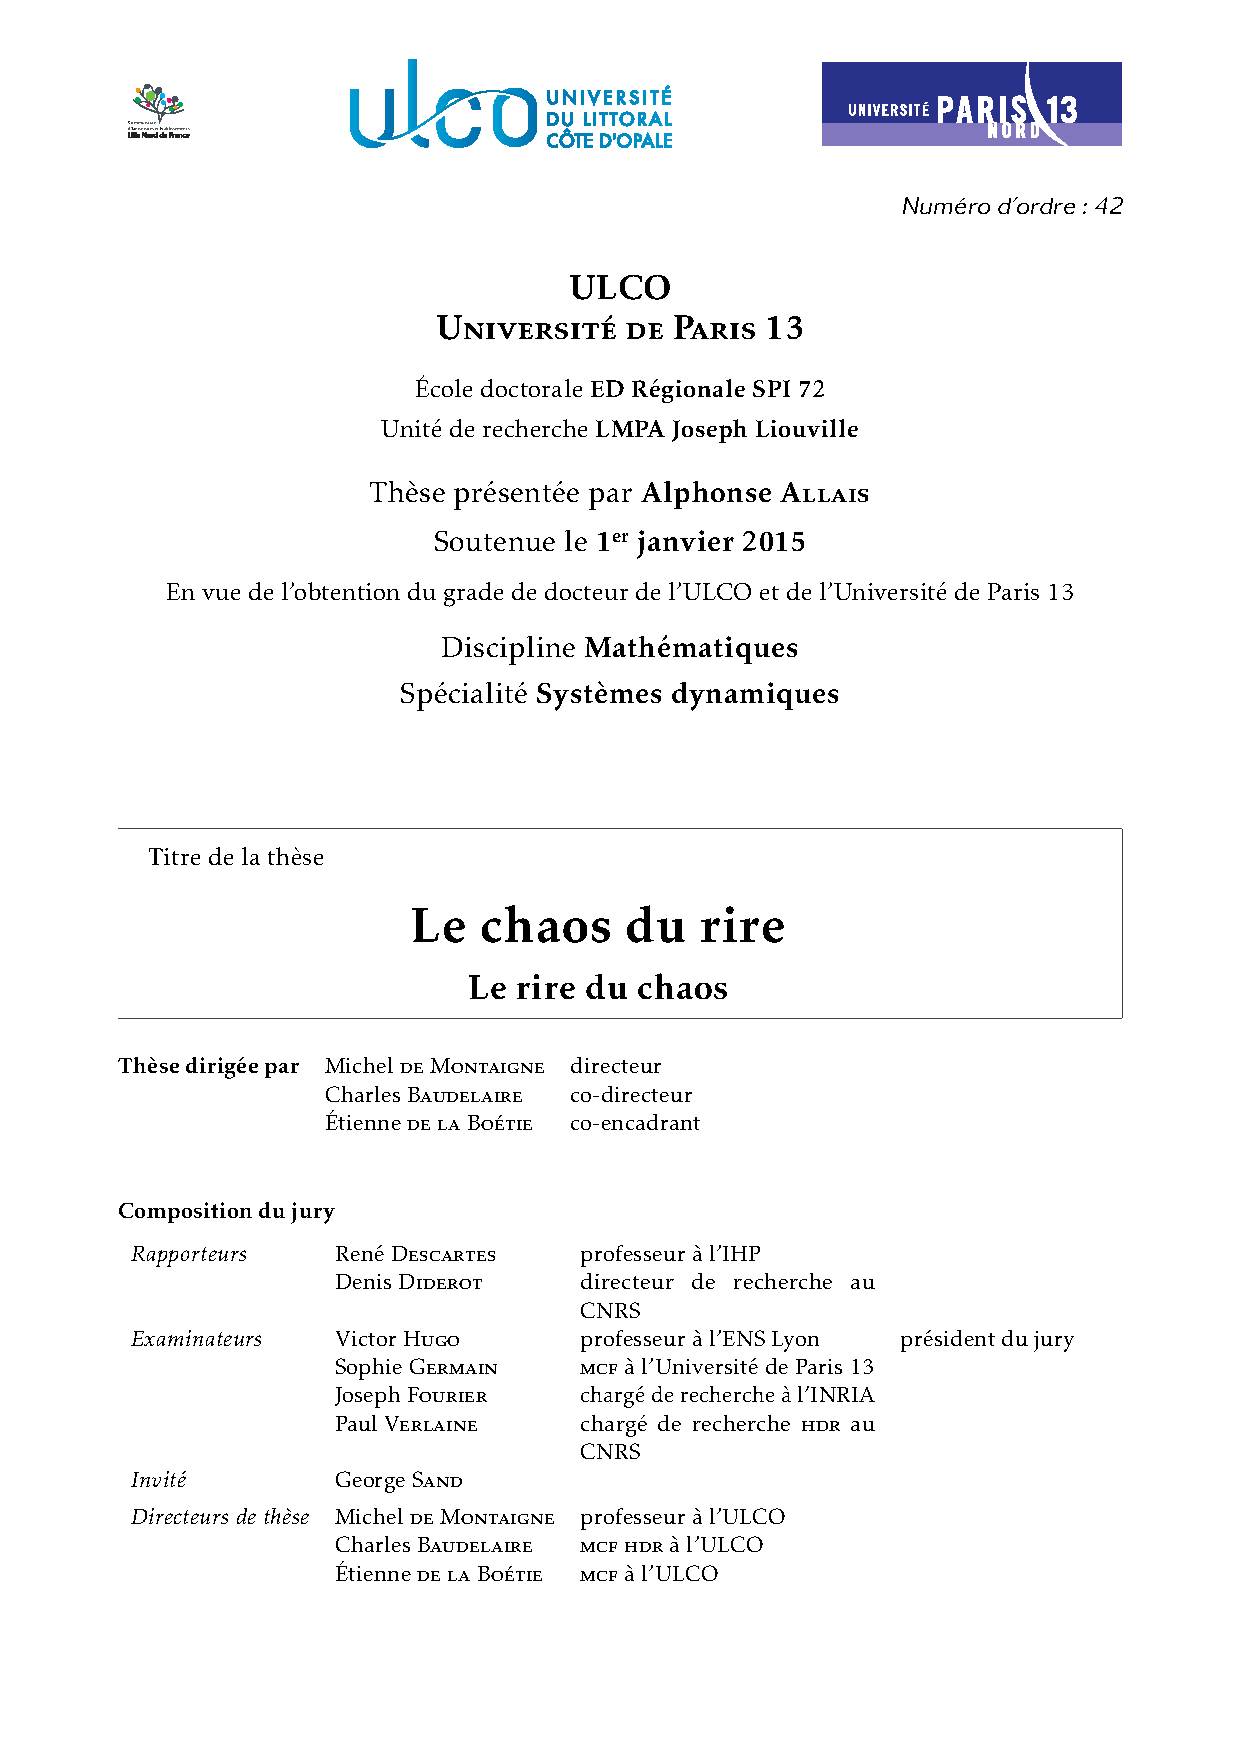
\includegraphics[bylabel=#2,width=#1\linewidth-2\fboxsep-2\fboxrule]{\c_@@_flatsample_string_tl/these}}%
    }{%
      \begin{dbwarning}{Copie~d'écran~manquante~!}{}
        Il~ devrait~ ici~ y~ avoir~ une~ copie\c_space_tl ~ d'écran.~ Cf.~
        \vref{wa-documentation-incomplete}~ pour~ plus~ de~ détails.
      \end{dbwarning}
    }
  }
  \NewDocumentCommand \screenshot { O{.45} m } {%
    \_@@_screenshot:nn {#1}{#2}
  }
}
%    \end{macrocode}
%
% In order to get rid of the warning "PDF inclusion: multiple pdfs with page
% group included in a single page" (see
% \url{http://tex.stackexchange.com/q/183149/18401}).
%    \begin{macrocode}
\pdfsuppresswarningpagegroup=1
%    \end{macrocode}
%
%    \begin{macrocode}
\cs_new_protected:Nn \_@@_meta:nn
{
    \bgroup%
    \normalfont
    \ttfamily%
    \textcolor{#1}{$\langle$\emph{#2}$\rangle$}%
    \egroup%
}
\AtBeginDocument{%
  \RenewDocumentCommand{\meta}{ O{meta} m } {
    \_@@_meta:nn {#1}{#2}
  }
}%
%    \end{macrocode}
%
% \subsection{Environments}
%
%    \begin{macrocode}
\NewTCBListing{preamblecode}{ O{} }{%
  codes,%
  drop~lifted~shadow,
  #1%
}
\NewTCBListing{bodycode}{ O{} }{%
  codes,%
  #1%
}
\NewTCBInputListing{\preamblesampleold}{ O{these.tex} m m }{%
  samples,
  drop~lifted~shadow,
  listing~file={\c_@@_treesample_string_tl/#1},
  listing~options={rangebeginprefix=\\,rangeendsuffix=\},#2},
  #3,
}%
\NewTCBInputListing{\preamblesample}{ m m m }{%
  samples,
  drop~lifted~shadow,
  listing~file={\c_@@_these_snippets_directory_tl/#1},
  listing~options={#2},
  #3,
}%
\NewTCBInputListing{\bodysampleold}{ O{these.tex} m m }{%
  samples,
  listing~file={\c_@@_treesample_string_tl/#1},
  listing~options={rangebeginprefix=\\,rangeendsuffix=\},#2},
  #3,
}%
\NewTCBInputListing{\bodysample}{ m m m }{%
  samples,
  listing~file={\c_@@_these_snippets_directory_tl/#1},
  listing~options={#2},
  #3,
}%
% \newtcbinputlisting{\preamblesample}[3][these.tex]{%
%   samples,
%   drop~lifted~shadow,
%   listing~file={\c_@@_treesample_string_tl/#1},
%   listing~options={rangebeginprefix=\\,rangeendsuffix=\},#2},
%   #3,
% }%
% \newtcbinputlisting{\bodysample}[3][these.tex]{%
%   samples,
%   listing~file={\c_@@_treesample_string_tl/#1},
%   listing~options={rangebeginprefix=\\,rangeendsuffix=\},#2},
%   #3,
% }%
%    \end{macrocode}
%
% \subsection{Theorems}
%
%    \begin{macrocode}
\tl_new:N \g_@@_number_within_tl
\tl_set:Nn \g_@@_number_within_tl {chapter}
\@ifclassloaded{gztarticle}{\tl_set:Nn \g_@@_number_within_tl {section}}{}%
\@ifclassloaded{nwejmart}{\tl_set:Nn \g_@@_number_within_tl {section}}{}%
%    \end{macrocode}
%
%    \begin{macrocode}
\newtcbtheorem[list~inside=dbwarninglist,number~within=\g_@@_number_within_tl,crefname={avertissement}{avertissements}]{dbwarning}{Avertissement}{%
  colback=red!5!white,
  colframe=red!75!black,
  dbtcb
}{wa}
%
\newtcbtheorem[list~inside=dbexamplelist,number~within=\g_@@_number_within_tl,crefname={exemple}{exemples}]{dbexample}{Exemple}{%
  colback=lime!5!white,
  colframe=lime!75!black,
  dbtcb
}{ex}
%
\newtcbtheorem[list~inside=dbremarklist,number~within=\g_@@_number_within_tl,crefname={remarque}{remarques}]{dbremark}{Remarque}{%
  colback=cyan!5!white,
  colframe=cyan!75!black,
  dbtcb
}{rq}
\newtcbtheorem[list~inside=dbfaqlist,number~within=\g_@@_number_within_tl,crefname={question}{questions}]{dbfaq}{Question}{%
  colback=lightgray!5!white,
  colframe=lightgray!75!black,
  fontupper=\itshape,
  dbtcb
}{faq}
\newtcbtheorem[list~inside=dbtabularlist,number~within=\g_@@_number_within_tl,crefname={tableau}{tableaux}]{dbtab}{Tableau}{%
  colback=purple!5!white,
  colframe=purple!75!black,
  fontupper=\itshape,
  dbtcb
}{tab}
%    \end{macrocode}
%
% \section{Macros for menu entries}
%
% The following code is borrowed from
% \href{http://tex.stackexchange.com/a/40637/18401}{Enrico Gregorio (egreg)}.
%    \begin{macrocode}
\NewDocumentCommand{\menuentry}{ O{} m }
  {
   \group_begin: % to segregate local changes to keys and font
   \keys_set:nn { menuentry } { #1 }
   \exp_args:NNx \seq_set_split:Nnn \l_menuentry_seq { \l_menuentry_inputsep_tl } { #2 }
   \tl_use:N \l_menuentry_font_tl
   \bool_set_false:N \l_tmpa_bool
   \seq_map_function:NN \l_menuentry_seq \menuentry_process:n
   \group_end:
  }
\NewDocumentCommand{\menuentryset} { m }
  { \keys_set:nn { menuentry } { #1 } }

\tl_new:N \l_menuentry_font_tl
\tl_new:N \l_menuentry_sep_tl
\tl_new:N \l_menuentry_inputsep_tl
\seq_new:N \l_menuentry_seq

\cs_new:Npn \menuentry_process:n #1
  {
   \bool_if:NTF \l_tmpa_bool
     { \l_menuentry_sep_tl }
     { \bool_set_true:N \l_tmpa_bool }
   \tl_if_empty:nTF { #1 } {EMPTY~ARG!} { #1 }
  }
\keys_define:nn { menuentry }
  {
   menufont .tl_set:N = \l_menuentry_font_tl ,
   menusep  .tl_set:N = \l_menuentry_sep_tl,
   inputsep .tl_set:N = \l_menuentry_inputsep_tl,
  }
\keys_set:nn { menuentry }
  {
   menufont = \sffamily ,
   menusep  = ${}\to{}$
 }%    \end{macrocode}
\menuentryset{inputsep=>}
%
% \section{Definitions specific to peticular classes or packages}
%
% \subsection{\Class{yathesis}}
%
%    \begin{macrocode}
\tl_const:Nn \c_@@_yat_class_name_tl {yathesis}
\tl_const:Nn \c_@@_configuration_directory_string_tl {configuration}
\tl_const:Nn \c_@@_configuration_file_string_tl {thesis.cfg}
\tl_const:Nn \c_@@_characteristics_file_string_tl {characteristics.tex}
\tl_const:Nn \c_@@_macros_file_file_string_tl {macros.tex}
\tl_const:Nn \c_@@_auxiliary_directory_string_tl {auxiliaires}
\tl_const:Nn \c_@@_glossary_file_string_tl {glossaire.tex}
\tl_const:Nn \c_@@_acronyms_file_string_tl {acronymes.tex}
\tl_const:Nn \c_@@_symbols_file_string_tl {symboles.tex}
\tl_const:Nn \c_@@_images_directory_string_tl {images}
\tl_const:Nn \c_@@_thesis_master_file_string_tl {these}
%    \end{macrocode}
%
% \begin{macro}{\yat}
% \begin{macro}{\yatpa}
% \begin{macro}{\yatcl}
%    \begin{macrocode}
\NewDocumentCommand \yat { }
{%
  \textsl{\textsf{\c_@@_yat_class_name_tl}}
}
\NewDocumentCommand \yatpa { }
{%
  \Package+{\c_@@_yat_class_name_tl}[\itshape][]\xspace
}
\NewDocumentCommand \yatcl { }
{%
  \texorpdfstring{\class+{\c_@@_yat_class_name_tl}[][][\itshape]\xspace}{yathesis}
}
\NewDocumentCommand \yatCl { }
{%
  \texorpdfstring{\Class+{\c_@@_yat_class_name_tl}[][][\itshape]\xspace}{classe yathesis}
}
%    \end{macrocode}
% \end{macro}
% \end{macro}
% \end{macro}
%
%    \begin{macrocode}
\NewDocumentCommand \configurationdirectory { }
{%
  \c_@@_configuration_directory_string_tl
}
\NewDocumentCommand \configurationfile { }
{%
  \c_@@_configuration_file_string_tl
}
\NewDocumentCommand \characteristicsfile { }
{%
  \c_@@_characteristics_file_string_tl
}
\NewDocumentCommand \macrosfile { }
{%
  \c_@@_macros_file_string_tl
}
\NewDocumentCommand \auxiliarydirectory { }
{%
  \c_@@_auxiliary_directory_string_tl
}
\NewDocumentCommand \glossaryfile { }
{%
  \c_@@_glossary_file_string_tl
}
\NewDocumentCommand \acronymsfile { }
{%
  \c_@@_acronyms_file_string_tl
}
\NewDocumentCommand \symbolsfile { }
{%
  \c_@@_symbols_file_string_tl
}
\NewDocumentCommand \imagesdirectory { }
{%
  \c_@@_images_directory_string_tl
}
\NewDocumentCommand \thesismasterfile { }
{%
  \c_@@_thesis_master_file_string_tl
}
%    \end{macrocode}
%
% \subsection{\Class{gzt}}
%
%    \begin{macrocode}
\tl_const:Nn \c_@@_gzt_class_name_tl {gzt}
\tl_const:Nn \c_@@_gztauthor_class_name_tl {gztarticle}
\tl_const:Nn \c_@@_journal_short_title_string_tl {Gazette}
\tl_const:Nn \c_@@_journal_title_string_tl {
  \c_@@_journal_short_title_string_tl{}~des~Math\'ematiciens%
}
%    \end{macrocode}
%
% \begin{macro}{\gzt}
% \begin{macro}{\gztcl}
%    \begin{macrocode}
% \NewDocumentCommand \gzt { s } {
%   \IfBooleanTF {#1}
%   {
%     \textit{\c_@@_journal_title_string_tl}
%   }
%   {
%     \textit{\c_@@_journal_short_title_string_tl}
%   }
% }
% \NewDocumentCommand \gztcl { }
% {%
%   \Class{\textsl{\texttt{\c_@@_gzt_class_name_tl}}}
% }
\NewDocumentCommand \gztauthor { }
{%
  \textsl{\texttt{\c_@@_gztauthor_class_name_tl}}
}
\NewDocumentCommand \gztauthorcl { }
{%
  \Class+[http://ctan.org/pkg/gzt]{\gztauthor}
}
%    \end{macrocode}
% \end{macro}
% \end{macro}
% \end{macro}
%
% \subsection{\Class{nwejm}}
%
%    \begin{macrocode}
\tl_const:Nn \c_@@_nwejm_class_name_tl {nwejm}
\tl_const:Nn \c_@@_nwejmauthor_class_name_tl {nwejmart}
%    \end{macrocode}
%
% \begin{macro}{\nwejm}
% \begin{macro}{\nwejmcl}
%    \begin{macrocode}
\ProvideDocumentCommand \nwejm { s } {
  \IfBooleanTF {#1}
  {
    \textit{\c_@@_journal_title_string_tl}
  }
  {
    \textit{\c_@@_journal_short_title_string_tl}
  }
}
\ProvideDocumentCommand \nwejmcl { }
{%
  \Class{\c_@@_nwejm_class_name_tl}
}
\NewDocumentCommand \nwejmauthor { }
{%
  \class[\c_@@_standard_url_tl\c_@@_nwejm_class_name_tl]{\c_@@_nwejmauthor_class_name_tl}
}
\NewDocumentCommand \nwejmauthorcl { }
{%
  \Class[\c_@@_standard_url_tl\c_@@_nwejm_class_name_tl]{\c_@@_nwejmauthor_class_name_tl}
}
%    \end{macrocode}
% \end{macro}
% \end{macro}
% \end{macro}
%
% We PDFdisable some commands in order to avoid troubles in bookmarks.
%    \begin{macrocode}
\pdfstringdefDisableCommands{%
  \let\textcolor\@gobble
  \def\yatcl{yathesis}
  \def\yatCl{classe~yathesis}
  \def\program#1{#1}
}
%    \end{macrocode}
% \end{macro}
% \end{macro}
% \end{macro}
%
% We switch to a \enquote{normal} category code régime.
%    \begin{macrocode}
\ExplSyntaxOff
%    \end{macrocode}
%
%    \begin{macrocode}
%</package>
%    \end{macrocode}
%
%    \begin{macrocode}
%<*xindy-style>
%    \end{macrocode}
%
%    \begin{macrocode}
;; (define-attributes ("example"))
;; (define-attributes ("definition"))
(define-attributes (("default" "definition" "example")))
(define-attributes ("textsf"))
(markup-locref :open "\hyperpage{" :close "}" :attr "default")
(markup-locref :open "\textbf{\hyperpage{" :close "}}" :attr "definition")
(markup-locref :open "\textit{\hyperpage{" :close "}}" :attr "textit")
(markup-locref :open "\textsf{\hyperpage{" :close "}}" :attr "textsf")
(markup-locref :open "\emph{\hyperpage{" :close "}}" :attr "example")

(markup-crossref-list :class "see" :open "\seelink{" :sep "; " :close "}{}")

(define-crossref-class "hyperindexformat")
(markup-crossref-list :class "hyperindexformat" :open
      "\hyperindexformat{" :sep "; " :close "}{}")

;; (merge-to "definition" "default" :drop)

(markup-locref :open "\hyperpage{" :close "}")
(markup-locref :open "\hyperpage{" :close "}" :attr "hyperpage")


(markup-keyword-list :open "\targetindexentry{" :close "}" )
(markup-keyword-list :open "\targetindexentryi{" :close "}" :depth 1)
(markup-keyword-list :open "\targetindexentryii{" :close "}" :depth 2)

(markup-index :open  "~n
% \bookmarksetup{open}
\begin{theindex}
  \providecommand*\lettergroupDefault[1]{}
  \providecommand*\lettergroup[1]{%
    \belowpdfbookmark{#1}{\csuse{DBD@index@symbolic@name}:#1}%
    \par\indexheading{#1}{\csuse{DBD@index@symbolic@name}}\par
    \nopagebreak
  }
  ~n"
  :close "~n~n\end{theindex}~n"
:tree)
%    \end{macrocode}
%
%    \begin{macrocode}
%</xindy-style>
%    \end{macrocode}
%
%    \begin{macrocode}
%<*xindy-style-chng>
%    \end{macrocode}
%
%    \begin{macrocode}
(define-crossref-class "hyperindexformat")
(markup-crossref-list :class "hyperindexformat" :open
      "\hyperindexformat{" :sep "; " :close "}{}")

(markup-locref :open "\hyperpage{" :close "}")

(markup-locref-list :sep ", ")
(markup-locclass-list :open "\hspace*{\fill}\nobreakspace" :close "" )

(define-attributes (("gobble" "default")))
(markup-locref  :open "\makeatletter\@gobble{" :close "}\makeatother" :attr "gobble")
% (markup-locclass-list :open "" :sep "")

% (markup-keyword-list :open "{\small " :close "}" )
% (markup-keyword-list :open "{\small " :close "}" :depth 1)
% (markup-keyword-list :open "{\small " :close "}" :depth 2)

(markup-index :open  "~n
\clearpage
\phantomsection
\begin{theindex}
  \small
  \providecommand*\lettergroupDefault[1]{}
  \providecommand*\lettergroup[1]{}
  ~n"
  :close "~n~n\end{theindex}~n"
:tree)
%    \end{macrocode}
%
%    \begin{macrocode}
%</xindy-style-chng>
%    \end{macrocode}
%
% \end{implementation}
%
% \PrintChanges
%
% \PrintIndex
\endinput

% Local Variables:
% mode: doctex
% eval: (doctex-mode)
% TeX-engine: xetex
% TeX-command-default: "TeX"
% TeX-master: t
% ispell-local-dictionary: "francais"
% End:
